\documentclass[conference]{IEEEtran}
\IEEEoverridecommandlockouts
% The preceding line is only needed to identify funding in the first footnote. If that is unneeded, please comment it out.
%Template version as of 6/27/2024

\usepackage[colorlinks=true, linkcolor=black, citecolor=blue, urlcolor=blue]{hyperref}

\usepackage{cite}
\usepackage{amsmath,amssymb,amsfonts}
\usepackage{algorithmic}
\usepackage{graphicx}
\usepackage{textcomp}
\usepackage{xcolor}
\def\BibTeX{{\rm B\kern-.05em{\sc i\kern-.025em b}\kern-.08em
	T\kern-.1667em\lower.7ex\hbox{E}\kern-.125emX}}
\begin{document}

%\title{Conference Paper Title*\\
	%{\footnotesize \textsuperscript{*}Note: Sub-titles are not captured for https://ieeexplore.ieee.org  and
		%should not be used}
	%\thanks{Identify applicable funding agency here. If none, delete this.}
	%}
%
%\author{\IEEEauthorblockN{1\textsuperscript{st} Given Name Surname}
	%\IEEEauthorblockA{\textit{dept. name of organization (of Aff.)} \\
		%\textit{name of organization (of Aff.)}\\
		%City, Country \\
		%email address or ORCID}
	%\and
	%\IEEEauthorblockN{2\textsuperscript{nd} Given Name Surname}
	%\IEEEauthorblockA{\textit{dept. name of organization (of Aff.)} \\
		%\textit{name of organization (of Aff.)}\\
		%City, Country \\
		%email address or ORCID}
	%\and
	%\IEEEauthorblockN{3\textsuperscript{rd} Given Name Surname}
	%\IEEEauthorblockA{\textit{dept. name of organization (of Aff.)} \\
		%\textit{name of organization (of Aff.)}\\
		%City, Country \\
		%email address or ORCID}
	%\and
	%\IEEEauthorblockN{4\textsuperscript{th} Given Name Surname}
	%\IEEEauthorblockA{\textit{dept. name of organization (of Aff.)} \\
		%\textit{name of organization (of Aff.)}\\
		%City, Country \\
		%email address or ORCID}
	%\and
	%\IEEEauthorblockN{5\textsuperscript{th} Given Name Surname}
	%\IEEEauthorblockA{\textit{dept. name of organization (of Aff.)} \\
		%\textit{name of organization (of Aff.)}\\
		%City, Country \\
		%email address or ORCID}
	%\and
	%\IEEEauthorblockN{6\textsuperscript{th} Given Name Surname}
	%\IEEEauthorblockA{\textit{dept. name of organization (of Aff.)} \\
		%\textit{name of organization (of Aff.)}\\
		%City, Country \\
		%email address or ORCID}
	%}

\title{Deriving IT Strategies from Times Higher Education Rank}
% \author{\textbf{[Hidden for double-blind review]}}
\author{\IEEEauthorblockN{
		Alfa Yohannis%\IEEEauthorrefmark{1}
		\IEEEauthorrefmark{2},
		Master Edison Sinaga%\IEEEauthorrefmark{1}%\IEEEauthorrefmark{3}
	}
	\IEEEauthorblockA{
		% \IEEEauthorrefmark{1}
		Department of Informatics\\
		Pradita University, Tangerang, Indonesia\\
		\IEEEauthorrefmark{2}alfa.ryano@pradita.ac.id}
	% 	% \IEEEauthorblockA{
		% 	% 	\IEEEauthorrefmark{2}Department of Computer Science\\
		% 	% 	University of York, York, United Kingdom}
}

\newcommand{\al}[1]{{\textbf{\color{blue} Al: #1}}}

\maketitle

\begin{abstract}
	This study explores the correlations among key metrics from the Times Higher Education (THE) rankings over a 10-year period to derive actionable IT strategies for universities. Using rigorous analysis, including Spearman's Rank Correlation, the research identifies the most influential variables affecting institutional performance, such as research and teaching scores, citations, and international outlook. The findings underscore the importance of aligning IT investments with these critical areas to enhance institutional rankings and competitiveness. Based on the analysis, targeted IT strategies are recommended to support the performance of higher education institutions based on the influential variables.
\end{abstract}

\begin{IEEEkeywords}
	IT Strategy, Higher Education, Times Higher Education Rankings, Correlation Analysis, Data-Driven Decision-Making
\end{IEEEkeywords}


\section{Introduction}


The role of Information Technology (IT) strategy has become increasingly significant across various sectors, including Higher Education \cite{hashim2021higher}. In an era where digital transformation drives innovation, IT strategies are crucial for achieving institutional goals, enhancing operational efficiency, and improving the quality of services provided \cite{rahmadi2024research}. Within the context of Higher Education, these strategies are vital for ensuring that institutions remain competitive in an increasingly dynamic academic environment \cite{fernandez2023digital}.

IT strategies in Higher Education are often developed through diverse methodologies, including strategic alignment with institutional goals, benchmarking against peer institutions, and leveraging frameworks such as enterprise architecture \cite{bianchi2023it}. These approaches aim to optimise the utilisation of technology to support academic excellence, enhance research outputs, and improve student engagement \cite{digitalsystems2022strategy}.

Moreover, global ranking systems, such as those provided by \textit{Times Higher Education (THE)}, introduce variables that significantly influence universities' positions in these rankings \cite{times2023methodology}. Factors such as research output, teaching quality, industry collaboration, and international outlook play a pivotal role in determining an institution’s rank \cite{times2022rankings}. By analysing the relationships between these variables, it becomes possible to identify which aspects should be prioritised within IT strategies to maximise their impact on institutional performance.



This study aims to explore the relationships among key variables highlighted by \textit{Times Higher Education (THE)} and how these insights can inform the development of effective IT strategies tailored to the needs of Higher Education institutions. Through an analysis of the correlations between these variables, patterns and dependencies are identified, highlighting critical areas of focus for IT investments. Based on this analysis, a set of IT strategies is proposed to specifically target improvements in the variables most significant to universities' performance.

This paper is structured into several sections. The Introduction highlights the significance of IT strategy in Higher Education, while the Related Work reviews studies on deriving such strategies, focusing on methodologies and the role of \textit{Times Higher Education} rankings. The Methodology describes the analysis of these rankings' variables. The Results and Discussion present key findings, followed by IT Strategy Recommendations offering actionable insights. Finally, the Conclusion and Future Work summarise the study's contributions and suggest future research directions.


\section{Literature Review}
\label{sec:literature_review}

The development of an Information Technology (IT) strategy is a critical process that aligns technology initiatives with organisational objectives. Various frameworks and methodologies have been proposed in the literature to aid this alignment, ensuring that IT contributes to achieving competitive advantage and operational efficiency.

\subsection{Frameworks for IT Strategy Development}

Drechsler and Weißschädel \cite{drechsler2018framework} proposed a framework tailored for small and medium enterprises (SMEs) to develop IT strategies. Their approach integrates theoretical foundations with empirical validation, ensuring practical relevance for organisations with limited resources. The framework emphasises iterative processes, allowing organisations to adapt their strategies dynamically as they grow and encounter new challenges.

El Alami and Belemlih \cite{elalami2021digital} explored the integration of IT governance and management frameworks, such as COBIT, to formulate a digital strategy. Their study highlights the importance of combining existing best practices to address emerging digital transformation needs. By focusing on governance, organisations can align IT objectives with overall business strategies effectively.

De Haes and Van Grembergen \cite{dehaes2009governance} emphasised the role of IT governance frameworks in supporting IT strategy development. They discussed the use of maturity models to assess and improve IT alignment with organisational goals. Their work also highlights the importance of executive-level involvement in IT decision-making processes.

\subsection{Alignment with Organisational Objectives}

Adama et al. \cite{adama2024alignment} examined theoretical frameworks that support the alignment of IT and business strategies to achieve sustained competitive advantage. They argue that IT strategy should not only support current business operations but also anticipate future market demands and technological advancements. This forward-looking approach ensures that IT remains a strategic asset rather than a mere operational tool.

Putra et al. \cite{putra2022trends} conducted a systematic review of IT strategy implementation trends across various sectors. Their findings underscore the challenges organisations face in aligning IT strategies with broader organisational objectives. Key barriers include resource constraints, resistance to change, and the complexity of integrating legacy systems with modern technologies.


\subsection{Challenges in IT Strategy Formulation}

Rahmadi \cite{rahmadi2024research} identified digital transformation as a key driver of IT strategy development. However, he also noted that many organisations struggle to keep pace with technological advancements. His research highlights the need for adaptive strategies that can evolve with changing market conditions and technological landscapes.

Fernández et al. \cite{fernandez2023digital} conducted a multivocal literature review of digital transformation initiatives in higher education. They emphasised the importance of stakeholder engagement in IT strategy development, noting that successful strategies often involve collaboration between IT departments, academic staff, and administrative leaders.

\subsection{Emerging Trends and Future Directions}

The increasing complexity of IT environments has led to the adoption of more sophisticated tools and methodologies for strategy development. For instance, machine learning and predictive analytics are now being used to forecast the impact of IT investments on organisational performance. These technologies enable more informed decision-making and greater agility in responding to market changes \cite{digitalsystems2022strategy}.


\subsection{Use of Rankings and Performance Metrics}

Performance metrics\footnote{The terms `metrics' and `variables' are used interchangeably.} play a pivotal role in shaping IT strategies, particularly in higher education institutions. Rankings such as those provided by Times Higher Education (THE) emphasize variables such as research output, teaching quality, and international collaboration as critical factors influencing university competitiveness. Integrating these metrics into IT strategies enables institutions to align their technological initiatives with objectives that enhance their global standing \cite{times2023methodology}.

Da Silva and Santos \cite{dasilva2014cobit} examined IT governance frameworks and their application in strategic planning, demonstrating that metrics derived from ranking systems like THE can serve as benchmarks for prioritising IT investments. This approach ensures that IT initiatives directly contribute to improving institutional rankings and overall performance.

Further exploration of the relationship between ranking metrics and strategic planning is provided by Uslu \cite{uslu2020university}, who analysed key indicators from international university rankings, including THE. Uslu's findings reveal how metrics such as research output, teaching quality, and international collaboration can inform institutional strategies aimed at enhancing competitiveness. By understanding the weight and impact of these indicators, universities can craft IT strategies that target specific areas for improvement, directly contributing to enhanced rankings.

A complementary perspective is offered by a study on university competitiveness through data analytics \cite{analytics2022competitiveness}, which proposed predictive models to assist universities in improving their performance in rankings like THE. These models leverage historical ranking data and institutional metrics to identify areas requiring focused improvement. The study underscores the importance of IT in enabling data-driven decision-making and strategic planning, ensuring that technology investments are directed towards metrics with the highest potential impact.

Although the direct linkage between THE metrics and IT strategy development is not always explicit, these studies collectively provide actionable insights. Universities can harness IT to implement strategies that enhance performance in areas such as research output, teaching excellence, and global collaboration—key drivers of improved ranking outcomes.

This research builds on these foundations by taking a unique approach. It examines THE metrics and variables over a longitudinal period of 10 or more years, providing a deeper understanding of their correlations and influence on institutional rankings. By identifying the most impactful variables, this study offers a framework for developing IT strategies that specifically address these critical areas. Such targeted strategies ensure that IT investments are optimally aligned with institutional objectives, maximising their impact on performance and ranking outcomes.


\section{Methodology}
\label{sec:methodology}

The research was performed quantitatively, with data collected through web scrapping. Python scripts were written to process, analyse, and visualise the collected data using its various libraries. 

\subsection{Data Collection and Cleaning}

The data scrapping was achieved by collecting universities' ranks and rank factors by scrapping scores from 2013 to 2023 in the Times Higher Education (THE) website \cite{the2024} and combining it with the data of university ranks obtained from Kaggle \cite{ONeil_2020}\footnote{The contribution of this dataset was minimal.}, producing more than 11-year data span with 711 universities involved. 

After collecting the necessary data, it underwent several data-cleaning steps to ensure it was ready for analysis. First, empty numeric values were filled using linear estimation, logarithmic estimation, etc., based on the coefficient of determination $R^{2}$ to estimate the missing values. The filled values were then normalized and added as a new column to the dataset. Secondly, empty non-numeric values were filled with `n/a' to help handle missing non-numeric values in the following steps.

Finally, unnecessary columns were removed to streamline the dataset, and only several columns were used in the analysis as variables. These variables were international outlook score, rank, citations score, overall score, industry income score, international students, research score, number of students, student-to-staff ratio, and teaching score. 

\subsection{Data Analysis}

Correlations were calculated between the variables. The analysis assessed the strength of the relationships using correlation coefficients, along with their statistical significance. Spearman's Rank Correlation Coefficient \cite{spearman1904general} was employed to ensure the robustness of the results, as it does not assume normality in the data distribution. The significance of the correlations was evaluated to determine whether the observed relationships were likely to have occurred by chance. A graph chart was used to help comprehend the data, that nodes represented the variables of THE and edges were the correlations between them. 

\begin{figure*}[t]
	\centering
	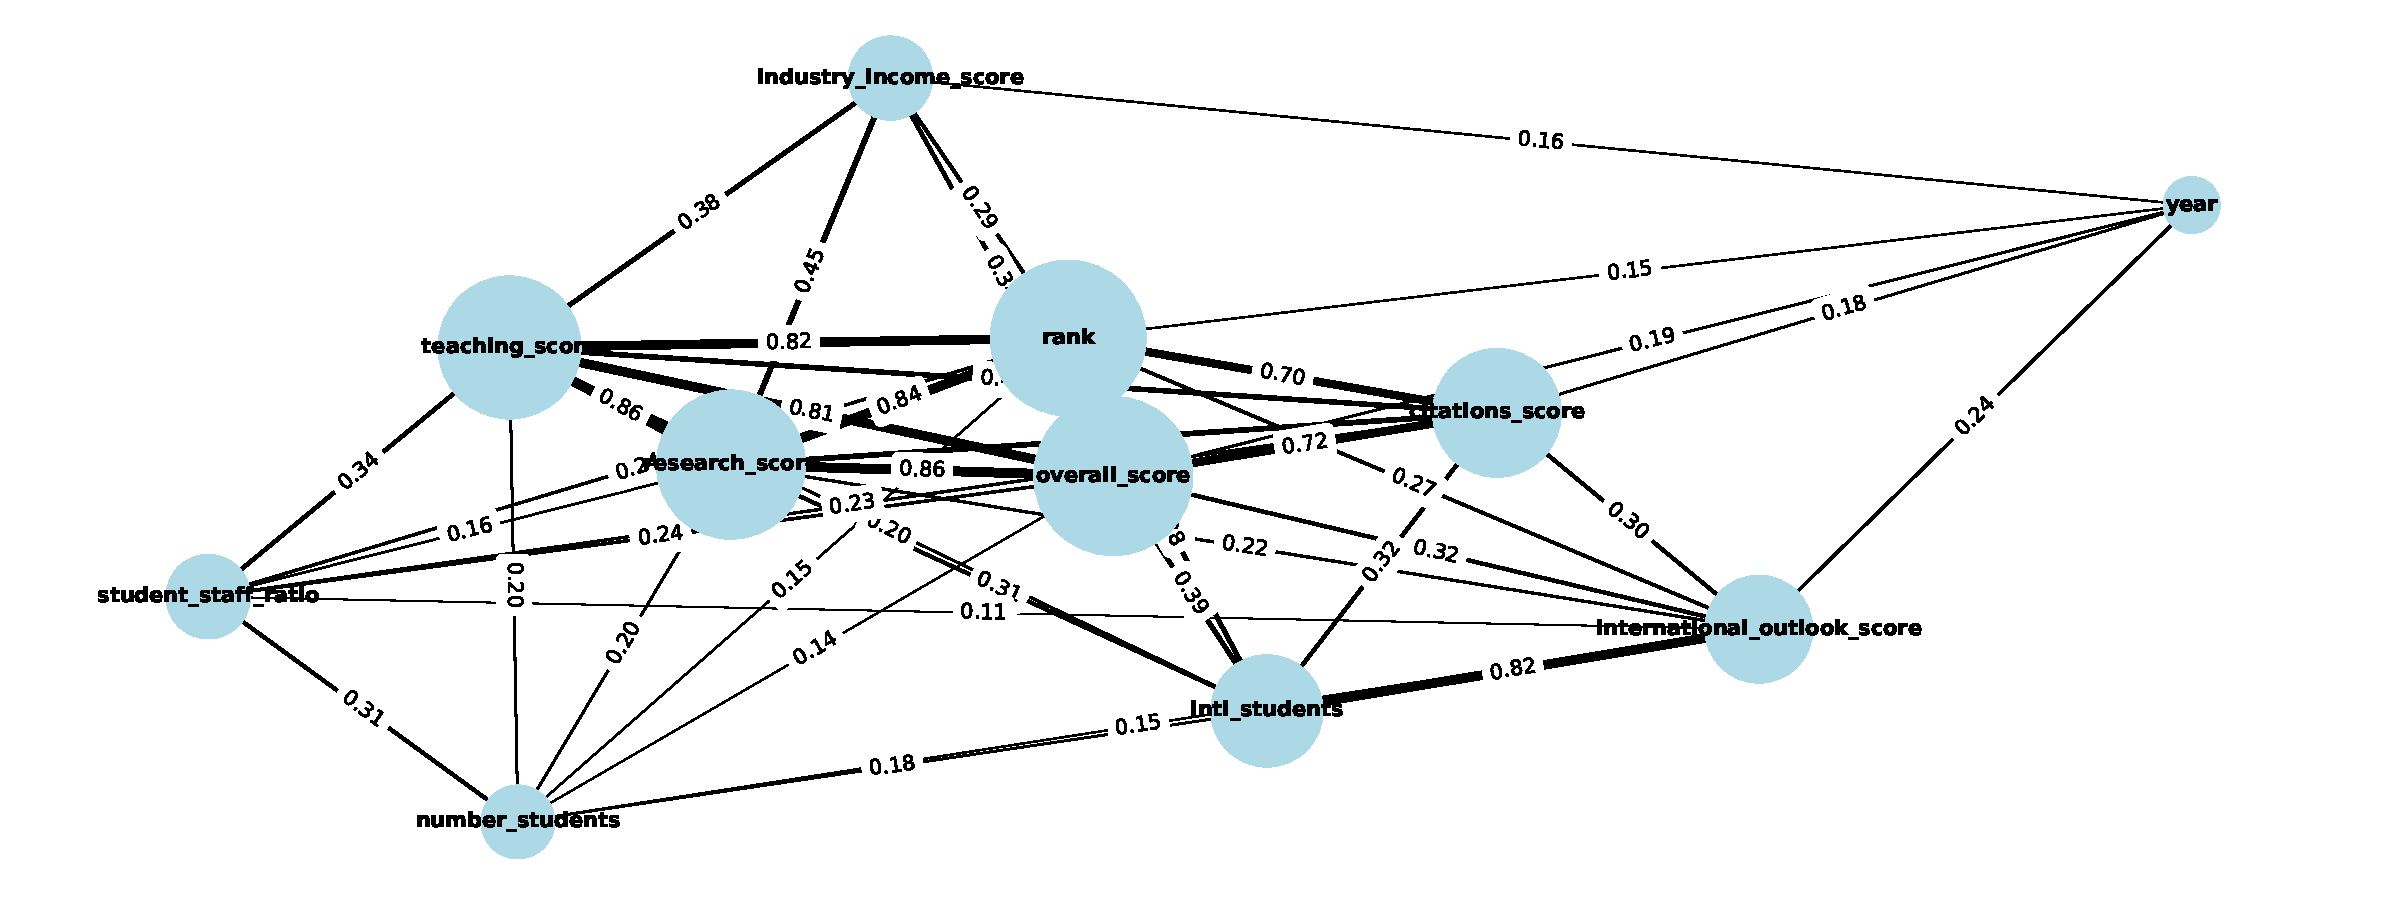
\includegraphics[width=\linewidth]{figures/correlation_graph.pdf}
	\caption{Correlation graph between the variables of Times Higher Education Rank. Correlations with }
	\label{fig:graf_citation}
\end{figure*}

\section{Results and Discussion}
This section examines the correlations among THE variables, including international outlook score, rank, citations score, overall score, industry income score, international students, research score, number of students, student-to-staff ratio, and teaching score. A summary of these correlations is presented in Fig. \ref{fig:graf_citation}. The graph highlights only significant correlations with a strength greater than 0.1. Additionally, the diameter of each node represents the variable's overall influence, calculated as the sum of its correlations with other variables.



\subsection{Analysis of Correlations with Rank}

The correlation analysis highlights key determinants influencing institutional rankings (Table \ref{tab:correlation_rank}). Among the examined variables, the \textit{overall score}, \textit{research score}, \textit{teaching score}, and \textit{citations score} exhibit the strongest negative correlations, underscoring their significant impact on rank. The \textit{overall score} ($r = -0.72$) and \textit{research score} ($r = -0.71$) emerge as the most influential factors, emphasizing their critical roles in driving institutional performance and competitiveness.

Moderate negative correlations are observed for \textit{international students} ($r = -0.34$) and \textit{international outlook score} ($r = -0.28$), suggesting that global engagement contributes meaningfully to rankings, albeit less prominently than performance metrics. The \textit{industry income score} ($r = -0.23$) also shows a negative association, albeit weaker, reflecting its relevance as a secondary factor.

On the other hand, positive correlations with \textit{year} ($r = 0.22$) and \textit{student-to-staff ratio} ($r = 0.08$) indicate that newer data and less favorable staff ratios are weakly associated with poorer rankings. The \textit{number of students} ($r = -0.03$, $p = 0.05$) demonstrates a negligible and borderline significant relationship, suggesting limited influence on rank outcomes.

These results reinforce the centrality of performance-driven metrics, particularly those related to research and teaching quality, in shaping institutional rankings. While internationalization factors add further depth, their impact is relatively modest compared to core academic indicators.

\begin{table}[h!]
	\centering
	\caption{Correlation Analysis Results for Institutional \textbf{Rank}}
	\label{tab:correlation_rank}
	\begin{tabular}{|l|r|r|}
		\hline
		\textbf{Variable} & \textbf{Correlation ($r$)} & \textbf{p-value} \\
		\hline
		Overall Score & -0.72 & 0.00 *** \\
		Research Score & -0.71 & 0.00 *** \\
		Teaching Score & -0.67 & 0.00 *** \\
		Citations Score & -0.67 & 0.00 *** \\
		International Students & -0.34 & 0.00 *** \\
		International Outlook Score & -0.28 & 0.00 *** \\
		Industry Income Score & -0.23 & 0.00 *** \\
		Year & 0.22 & 0.00 *** \\
		Student-to-Staff Ratio & 0.08 & 0.00 *** \\
		Number of Students & -0.03 & 0.05 * \\
		\hline
	\end{tabular}
\end{table}

\subsection{Analysis of Correlations with Overall Score}

The correlation analysis highlights key factors associated with the \textit{overall score}, emphasizing its role as a comprehensive measure of institutional performance (Table \ref{tab:correlation_overall}). Among the variables examined, the \textit{research score} ($r = 0.91$) and \textit{teaching score} ($r = 0.88$) exhibit the strongest positive correlations, underscoring the importance of academic and research excellence in achieving higher overall scores. These metrics are critical focal points for enhancing institutional performance.

The \textit{rank} ($r = -0.72$) demonstrates a strong negative correlation, indicating that higher overall scores are associated with better rankings (lower numerical values). This finding highlights the integral relationship between comprehensive institutional performance and competitive standings.

Moderate correlations are observed for \textit{citations score} ($r = 0.68$), \textit{international students} ($r = 0.37$), \textit{industry income score} ($r = 0.30$), and \textit{international outlook score} ($r = 0.30$). These metrics suggest that impactful research, global engagement, and industry collaborations play substantial roles in shaping the overall institutional score.

Weaker correlations include \textit{student-to-staff ratio} ($r = -0.19$), \textit{year} ($r = 0.13$), and \textit{number of students} ($r = 0.05$). These findings indicate limited direct influence on the overall score, though maintaining favorable ratios and engaging large student bodies remain important for broader institutional objectives.

\begin{table}[h!]
	\centering
	\caption{Correlation Analysis Results for \textbf{Overall} Score}
	\label{tab:correlation_overall}
	\begin{tabular}{|l|r|r|}
		\hline
		\textbf{Variable} & \textbf{Correlation ($r$)} & \textbf{p-value} \\
		\hline
		Research Score & 0.91 & 0.00 *** \\
		Teaching Score & 0.88 & 0.00 *** \\
		Rank & -0.72 & 0.00 *** \\
		Citations Score & 0.68 & 0.00 *** \\
		International Students & 0.37 & 0.00 *** \\
		Industry Income Score & 0.30 & 0.00 *** \\
		International Outlook Score & 0.30 & 0.00 *** \\
		Student-to-Staff Ratio & -0.19 & 0.00 *** \\
		Year & 0.13 & 0.00 *** \\
		Number of Students & 0.05 & 0.00 *** \\
		\hline
	\end{tabular}
\end{table}



\subsection{Analysis of Correlations with Research Score}

The correlation analysis reveals critical factors that contribute to the \textit{research score}, highlighting its central role in institutional performance (Table \ref{tab:correlation_research}). Among the examined variables, the \textit{teaching score} ($r = 0.92$) and \textit{overall score} ($r = 0.91$) exhibit the strongest positive correlations, emphasizing their close alignment with research activities. Enhancing both teaching and overall institutional quality directly supports improvements in research performance.

The \textit{rank} ($r = -0.71$) demonstrates a strong negative correlation, reaffirming the inverse relationship where higher research scores correspond to better rankings (lower rank values). This underscores the integral role of research excellence in achieving competitive standings.

Moderate correlations are observed for \textit{citations score} ($r = 0.45$), \textit{industry income score} ($r = 0.40$), and \textit{international students} ($r = 0.30$). These findings suggest that impactful research outputs, industry partnerships, and global engagement significantly influence research scores. \textit{International outlook score} ($r = 0.21$) also reflects the contribution of internationalization, albeit to a lesser extent.

Weaker correlations include \textit{student-to-staff ratio} ($r = -0.14$), \textit{number of students} ($r = 0.11$), and \textit{year} ($r = 0.06$). These metrics, while statistically significant, show limited direct impact on research performance. Efforts to optimize these factors may still provide ancillary benefits to institutional quality.

\begin{table}[h!]
	\centering
	\caption{Correlation Analysis Results for \textbf{Research} Score}
	\label{tab:correlation_research}
	\begin{tabular}{|l|r|r|}
		\hline
		\textbf{Variable} & \textbf{Correlation ($r$)} & \textbf{p-value} \\
		\hline
		Teaching Score & 0.92 & 0.00 *** \\
		Overall Score & 0.91 & 0.00 *** \\
		Rank & -0.71 & 0.00 *** \\
		Citations Score & 0.45 & 0.00 *** \\
		Industry Income Score & 0.40 & 0.00 *** \\
		International Students & 0.30 & 0.00 *** \\
		International Outlook Score & 0.21 & 0.00 *** \\
		Student-to-Staff Ratio & -0.14 & 0.00 *** \\
		Number of Students & 0.11 & 0.00 *** \\
		Year & 0.06 & 0.00 *** \\
		\hline
	\end{tabular}
\end{table}


\subsection{Analysis of Correlations with Citations Score}

The correlation analysis identifies key factors associated with the \textit{citations score}, highlighting its significance as a measure of research impact (Table \ref{tab:correlation_citations}). Among the variables examined, the \textit{overall score} ($r = 0.68$) exhibits the strongest positive correlation, underscoring the alignment between high overall institutional performance and research impact through citations. The \textit{rank} ($r = -0.67$) shows a strong negative correlation, reflecting the role of citations in improving institutional rankings (lower rank values).

Moderate positive correlations are observed for \textit{research score} ($r = 0.45$), \textit{teaching score} ($r = 0.44$), \textit{international outlook score} ($r = 0.33$), and \textit{international students} ($r = 0.30$). These findings suggest that impactful research, quality teaching, and global engagement contribute significantly to citation performance.

Weaker correlations include \textit{year} ($r = 0.18$) and \textit{student-to-staff ratio} ($r = -0.13$), indicating limited direct influence. The \textit{number of students} ($r = -0.03$, $p = 0.03$) shows a negligible and weakly significant negative relationship, while \textit{industry income score} ($r = -0.01$, $p = 0.62$) demonstrates no significant correlation, highlighting its limited relevance to citations.

\begin{table}[h!]
	\centering
	\caption{Correlation Analysis Results for \textbf{Citations} Score}
	\label{tab:correlation_citations}
	\begin{tabular}{|l|r|r|}
		\hline
		\textbf{Variable} & \textbf{Correlation ($r$)} & \textbf{p-value} \\
		\hline
		Overall Score & 0.68 & 0.00 *** \\
		Rank & -0.67 & 0.00 *** \\
		Research Score & 0.45 & 0.00 *** \\
		Teaching Score & 0.44 & 0.00 *** \\
		International Outlook Score & 0.33 & 0.00 *** \\
		International Students & 0.30 & 0.00 *** \\
		Year & 0.18 & 0.00 *** \\
		Student-to-Staff Ratio & -0.13 & 0.00 *** \\
		Number of Students & -0.03 & 0.03 ** \\
		Industry Income Score & -0.01 & 0.62 \\
		\hline
	\end{tabular}
\end{table}


\subsection{Analysis of Correlations with Industry Income Score}

The correlation analysis identifies key factors associated with the \textit{industry income score} (Table \ref{tab:correlation_industry_income}), emphasizing its relevance to institutional partnerships and financial sustainability. Among the variables examined, the \textit{research score} ($r = 0.40$) and \textit{teaching score} ($r = 0.34$) exhibit the strongest positive correlations. These findings highlight the importance of robust research and teaching activities in attracting industry partnerships and increasing income from external sources.

The \textit{overall score} ($r = 0.30$) also shows a moderate positive correlation, reflecting the role of comprehensive institutional performance in driving industry income. The \textit{rank} ($r = -0.23$) displays a negative correlation, indicating that institutions with higher industry income scores tend to have better rankings (lower numerical values).

Weaker positive correlations are observed for \textit{year} ($r = 0.10$) and \textit{student-to-staff ratio} ($r = 0.05$), suggesting limited direct influence on the \textit{industry income score}. The \textit{number of students} ($r = -0.03$, $p = 0.06$) demonstrates a negligible and borderline significant negative relationship, while \textit{international students} ($r = -0.02$, $p = 0.17$), \textit{international outlook score} ($r = -0.02$, $p = 0.19$), and \textit{citations score} ($r = -0.01$, $p = 0.62$) show no significant correlations, indicating minimal relevance to industry income.

\begin{table}[h!]
	\centering
	\caption{Correlation Analysis Results for \textbf{Industry Income} Score}
	\label{tab:correlation_industry_income}
	\begin{tabular}{|l|r|r|}
		\hline
		\textbf{Variable} & \textbf{Correlation ($r$)} & \textbf{p-value} \\
		\hline
		Research Score & 0.40 & 0.00 *** \\
		Teaching Score & 0.34 & 0.00 *** \\
		Overall Score & 0.30 & 0.00 *** \\
		Rank & -0.23 & 0.00 *** \\
		Year & 0.10 & 0.00 *** \\
		Student-to-Staff Ratio & 0.05 & 0.00 *** \\
		Number of Students & -0.03 & 0.06 * \\
		International Students & -0.02 & 0.17 \\
		International Outlook Score & -0.02 & 0.19 \\
		Citations Score & -0.01 & 0.62 \\
		\hline
	\end{tabular}
\end{table}

\subsection{Analysis of Correlations with International Outlook Score}

The correlation analysis highlights the factors associated with the \textit{international outlook score} (Table \ref{tab:correlation_international_outlook}), emphasizing its role in reflecting global engagement and diversity. Among the variables examined, the \textit{international students} percentage ($r = 0.80$) exhibits the strongest positive correlation, underscoring the direct relationship between student diversity and an institution's international outlook.

Moderate positive correlations are observed for the \textit{citations score} ($r = 0.33$), \textit{overall score} ($r = 0.30$), and \textit{rank} ($r = -0.28$), indicating that institutions with higher research impact, comprehensive performance, and better rankings tend to have stronger international engagement. The \textit{year} ($r = 0.25$) also shows a moderate correlation, reflecting potential trends in increasing global focus over time.

Weaker correlations include \textit{research score} ($r = 0.21$), \textit{number of students} ($r = -0.18$), \textit{teaching score} ($r = 0.05$), and \textit{student-to-staff ratio} ($r = 0.04$). These findings suggest limited but significant influences on the international outlook score. The \textit{industry income score} ($r = -0.02$, $p = 0.19$) demonstrates no significant correlation, highlighting its minimal relevance to this metric.

\begin{table}[h!]
	\centering
	\caption{Correlation Analysis Results for \textbf{International Outlook} Score}
	\label{tab:correlation_international_outlook}
	\begin{tabular}{|l|r|r|}
		\hline
		\textbf{Variable} & \textbf{Correlation ($r$)} & \textbf{p-value} \\
		\hline
		International Students & 0.80 & 0.00 *** \\
		Citations Score & 0.33 & 0.00 *** \\
		Overall Score & 0.30 & 0.00 *** \\
		Rank & -0.28 & 0.00 *** \\
		Year & 0.25 & 0.00 *** \\
		Research Score & 0.21 & 0.00 *** \\
		Number of Students & -0.18 & 0.00 *** \\
		Teaching Score & 0.05 & 0.00 *** \\
		Student-to-Staff Ratio & 0.04 & 0.01 *** \\
		Industry Income Score & -0.02 & 0.19 \\
		\hline
	\end{tabular}
\end{table}

\subsection{Analysis of Correlations with Number of Students}

The correlation analysis highlights factors associated with the \textit{number of students} (Table \ref{tab:correlation_number_students}), emphasizing its role in shaping institutional dynamics. Among the variables examined, the \textit{student-to-staff ratio} ($r = 0.26$) exhibits the strongest positive correlation, suggesting that institutions with larger student populations tend to have higher student-to-staff ratios.

Moderate negative correlations are observed for \textit{international students} ($r = -0.21$) and \textit{international outlook score} ($r = -0.18$), indicating that institutions with larger student populations may have a relatively smaller proportion of international engagement. 

Weaker correlations include \textit{research score} ($r = 0.11$), \textit{teaching score} ($r = 0.11$), and \textit{overall score} ($r = 0.05$), suggesting limited direct influence on institutional performance metrics. Minimal negative correlations are noted for \textit{citations score} ($r = -0.03$, $p = 0.03$), \textit{rank} ($r = -0.03$, $p = 0.05$), and \textit{industry income score} ($r = -0.03$, $p = 0.06$), indicating borderline significant relationships. The \textit{year} ($r = 0.02$, $p = 0.16$) demonstrates negligible relevance.

\begin{table}[h!]
	\centering
	\caption{Correlation Analysis Results for \textbf{Number of Students}}
	\label{tab:correlation_number_students}
	\begin{tabular}{|l|r|r|}
		\hline
		\textbf{Variable} & \textbf{Correlation ($r$)} & \textbf{p-value} \\
		\hline
		Student-to-Staff Ratio & 0.26 & 0.00 *** \\
		International Students & -0.21 & 0.00 *** \\
		International Outlook Score & -0.18 & 0.00 *** \\
		Research Score & 0.11 & 0.00 *** \\
		Teaching Score & 0.11 & 0.00 *** \\
		Overall Score & 0.05 & 0.00 *** \\
		Citations Score & -0.03 & 0.03 ** \\
		Rank & -0.03 & 0.05 * \\
		Industry Income Score & -0.03 & 0.06 * \\
		Year & 0.02 & 0.16 \\
		\hline
	\end{tabular}
\end{table}


\subsection{Analysis of Correlations with Student-to-Staff Ratio}

The correlation analysis highlights factors associated with the \textit{student-to-staff ratio} (Table \ref{tab:correlation_student_staff_ratio}), emphasizing its role as an indicator of educational quality and institutional resources. Among the variables examined, the \textit{number of students} ($r = 0.26$) exhibits the strongest positive correlation, suggesting that larger student populations tend to be associated with higher student-to-staff ratios.

Moderate negative correlations are observed for the \textit{teaching score} ($r = -0.24$) and \textit{overall score} ($r = -0.19$), indicating that institutions with lower student-to-staff ratios often achieve better teaching and overall performance metrics. Additional negative correlations are noted for the \textit{research score} ($r = -0.14$), \textit{citations score} ($r = -0.13$), and \textit{international students} ($r = -0.09$), reflecting the association between lower ratios and improved research impact and international diversity.

Weaker positive correlations are observed for \textit{rank} ($r = 0.08$), \textit{industry income score} ($r = 0.05$), and \textit{international outlook score} ($r = 0.04$, $p = 0.01$), suggesting limited direct influence on the student-to-staff ratio. Minimal correlation is observed for \textit{year} ($r = 0.01$, $p = 0.37$), indicating negligible relevance to temporal trends.

\begin{table}[h!]
	\centering
	\caption{Correlation Analysis Results for \textbf{Student-to-Staff Ratio}}
	\label{tab:correlation_student_staff_ratio}
	\begin{tabular}{|l|r|r|}
		\hline
		\textbf{Variable} & \textbf{Correlation ($r$)} & \textbf{p-value} \\
		\hline
		Number of Students & 0.26 & 0.00 *** \\
		Teaching Score & -0.24 & 0.00 *** \\
		Overall Score & -0.19 & 0.00 *** \\
		Research Score & -0.14 & 0.00 *** \\
		Citations Score & -0.13 & 0.00 *** \\
		International Students & -0.09 & 0.00 *** \\
		Rank & 0.08 & 0.00 *** \\
		Industry Income Score & 0.05 & 0.00 *** \\
		International Outlook Score & 0.04 & 0.01 *** \\
		Year & 0.01 & 0.37 \\
		\hline
	\end{tabular}
\end{table}



\subsection{Analysis of Correlations with Year}

The correlation analysis highlights factors associated with the \textit{year} (Table \ref{tab:correlation_year}), providing insights into temporal trends and their relationships with institutional metrics. Among the variables examined, the \textit{international outlook score} ($r = 0.25$) exhibits the strongest positive correlation, reflecting an increasing focus on global engagement over time.

Moderate positive correlations are observed for \textit{rank} ($r = 0.22$), \textit{citations score} ($r = 0.18$), and \textit{overall score} ($r = 0.13$). These findings suggest that institutional performance metrics and research impact have gradually improved in recent years, influencing rankings and overall outcomes.

Weaker correlations include \textit{industry income score} ($r = 0.10$), \textit{international students} ($r = 0.10$), and \textit{research score} ($r = 0.06$), indicating limited but notable associations with temporal trends. Minimal correlations are observed for \textit{number of students} ($r = 0.02$, $p = 0.16$), \textit{student-to-staff ratio} ($r = 0.01$, $p = 0.37$), and \textit{teaching score} ($r = 0.00$, $p = 0.88$), highlighting their negligible relationship with the year.

\begin{table}[h!]
	\centering
	\caption{Correlation Analysis Results for \textbf{Year}}
	\label{tab:correlation_year}
	\begin{tabular}{|l|r|r|}
		\hline
		\textbf{Variable} & \textbf{Correlation ($r$)} & \textbf{p-value} \\
		\hline
		International Outlook Score & 0.25 & 0.00 *** \\
		Rank & 0.22 & 0.00 *** \\
		Citations Score & 0.18 & 0.00 *** \\
		Overall Score & 0.13 & 0.00 *** \\
		Industry Income Score & 0.10 & 0.00 *** \\
		International Students & 0.10 & 0.00 *** \\
		Research Score & 0.06 & 0.00 *** \\
		Number of Students & 0.02 & 0.16 \\
		Student-to-Staff Ratio & 0.01 & 0.37 \\
		Teaching Score & 0.00 & 0.88 \\
		\hline
	\end{tabular}
\end{table}



\subsection{Analysis of Variables by Total Influence}

The analysis of total influence highlights the hierarchical significance of various factors in determining outcomes (Table \ref{tab:total_influence}). Among the evaluated variables, the \textit{research score} demonstrates the highest total influence (8.29), followed closely by the \textit{teaching score} (7.65) and \textit{citations score} (6.34). These results underscore the predominant role of performance-driven metrics in shaping institutional success. 

Notably, internationalization-related variables such as \textit{international students} (5.29) and \textit{international outlook score} (4.68) have relatively lower influences, reflecting their supportive but secondary role in influencing outcomes.

Factors like \textit{industry income score} (2.76), \textit{year} (1.98), and \textit{student-to-staff ratio} (1.93) display the least influence, suggesting limited direct impact on the evaluated outcomes. The \textit{number of students} (1.74) shows a negligible normalized influence, marking it as the least impactful variable in the analysis.

\begin{table}[h!]
	\centering
	\caption{Variables Ordered by \textbf{Total Influence}}
	\label{tab:total_influence}
	\begin{tabular}{|l|r|r|}
		\hline
		\textbf{Variable} & \textbf{Total Influence} & \textbf{Normalized Influence} \\
		\hline
		Overall Score & 8.97 & 1.00 \\
		Research Score & 8.29 & 0.90 \\
		Rank & 7.66 & 0.82 \\
		Teaching Score & 7.65 & 0.82 \\
		Citations Score & 6.34 & 0.64 \\
		International Students & 5.29 & 0.49 \\
		International Outlook Score & 4.68 & 0.41 \\
		Industry Income Score & 2.76 & 0.14 \\
		Year & 1.98 & 0.03 \\
		Student-to-Staff Ratio & 1.93 & 0.03 \\
		Number of Students & 1.74 & 0.00 \\
		\hline
	\end{tabular}
\end{table}


\section{IT Strategy Recommendation}

In this section, we recommend some IT strategies for universities derived from the results of the correlation analysis. 

\begin{enumerate}
	\item \textbf{Enhance Research and Teaching Capabilities}: Given the strong correlations between \textit{research score} (\(r = 0.91\)) and \textit{teaching score} (\(r = 0.88\)) with the \textit{overall score}, universities should prioritize IT systems that support research and teaching excellence. Advanced research management systems should be implemented to track, evaluate, and promote high-quality research output. Additionally, e-learning platforms and virtual labs can enhance teaching quality and provide students with innovative learning experiences. Data analytics tools can also play a significant role in measuring the effectiveness of teaching methods and improving curriculum design.
	
	\item \textbf{Strengthen Citation and Research Impact}: The correlation between \textit{citations score} (\(r = 0.68\)) and \textit{overall score} highlights the importance of research visibility. Universities can leverage open-access repositories and IT systems to make research outputs widely accessible. Bibliometric tools should be employed to identify and promote impactful publications, while collaborative platforms can facilitate inter-institutional and cross-disciplinary research projects, further strengthening research impact.
	
	
	
	\item \textbf{Focus on Internationalization Strategies}: International engagement is supported by the correlations for \textit{international outlook score} (\(r = 0.30\)) and \textit{international students} (\(r = 0.37\)). Universities should develop international student portals equipped with tailored resources for recruitment and support. Multilingual IT systems can cater to a diverse audience, while virtual exchange programs and online collaborations with global institutions can enhance international presence and connectivity.
	
	\item \textbf{Optimize Industry Collaborations}: The moderate correlation between the \textit{industry income score} and \textit{research score} (\(r = 0.40\)) underscores the need for IT strategies focused on strengthening industry collaborations. Relationship management systems can help manage partnerships with industries effectively. IT platforms should support applied research and technology transfer activities, and dedicated online systems can promote internship and placement programs, bridging academia and industry.
	
	\item \textbf{Provide Scalable Resource Management}: The correlations between \textit{number of students} and \textit{student-to-staff ratio} (\(r = 0.26\)) indicate that growing student populations often lead to higher ratios, potentially affecting teaching quality and resource allocation. IT strategies should focus on scalable resource management systems, such as integrated ERP platforms, to balance student growth with faculty and infrastructure needs. Predictive analytics can forecast enrollment trends, aligning recruitment and resource planning to maintain optimal ratios and teaching outcomes. Digital platforms for hybrid or online teaching can also alleviate the pressure of high student-to-staff ratios by enabling more efficient use of resources.
	
	\item \textbf{Enhance the Experience of International Students}: The negative correlations between \textit{number of students} and \textit{international students} (\(r = -0.21\)) and \textit{international outlook score} (\(r = -0.18\)) highlight potential challenges in maintaining international diversity as student numbers grow. Universities can use IT systems to enhance the experience of international students through personalized support platforms and targeted global recruitment tools.
	
	\item \textbf{Adopt a Long-Term Digital Strategy}: The analysis of correlations between \textit{year} and institutional metrics reveals generally weak relationships, suggesting that improvements in these areas require long-term strategic efforts. The impact of strategies will be realized over extended periods, requiring consistent investment and adaptation to evolving trends.
\end{enumerate}

\section{Conclusions}

The analysis of correlations and total influences among various institutional performance metrics provides a robust foundation for developing targeted IT strategies for universities. Key findings highlight the pivotal role of research and teaching capabilities in enhancing overall institutional performance and rankings. Metrics such as \textit{citations score}, \textit{international outlook score}, and \textit{industry income score} further underscore the importance of visibility, global engagement, and collaborative efforts with industry partners. Operational metrics, while exhibiting relatively lower influence, still offer avenues for improving efficiency and resource management through data-driven decision-making and modern IT infrastructure. These insights culminate in strategic recommendations aimed at leveraging IT systems to optimize research, teaching, internationalization, and industry collaborations. For future work, further analysis can be conducted to explore the evolving correlations over time and their implications on institutional strategy. Expanding the scope of data to include diverse universities across regions can also enhance the generalizability and impact of these findings. 


\section*{Acknowledgement}

In this research, Artificial Intelligence (AI) played a pivotal role by assisting in the development of the script for scraping, data analysis, and summarization. The structure and flow of this paper were drafted by the authors, while AI contributed to generating the written content, grammar checking, rewording, and sentencing. Finally, the authors refined and polished the paper to ensure clarity, coherence, and alignment with the research objectives.

\bibliography{references}
\bibliographystyle{IEEEtran}

\end{document}
